% vim: set tw=78 sts=2 sw=2 ts=8 aw et ai:

\subsection{Standard library}

In order for the wireless sensor nodes to be usefull they will have to be
programmed to do a certain task. For this, Hive provides an API. It allows
common tasks like scheduling a timer or creating sockets. 

This API provided by Hive is platform agnostic. The code is loadable in the
simulator as plugin using libdl. When used on a physical node, the plugin must
provide only a load rutine. When ran on the simulator platform, the plugin
should also provide a start, stop and unload rutine.

\subsection{Networking}

Hive provides an API similar to the BSD sockets one. The functions name are
all appended with sys so they don't collide with the ones from glibc. It
contains just a small subset of BSD sockets API, but it will be extended if
it will be needed.
\begin{lstlisting}
sys_socket(int type, int protocol);
sys_sendto(int sock, char *buff, int size, sockaddr *to)
sys_recvfrom(int sock, char *buff, int size, sockaddr *from);
\end{lstlisting}
The plugin needs to specify the protocol used only when the socket is created,
but for all subsequent calls this will be handled by internal systems. 

\begin{figure}[htb]
  \begin{center}
    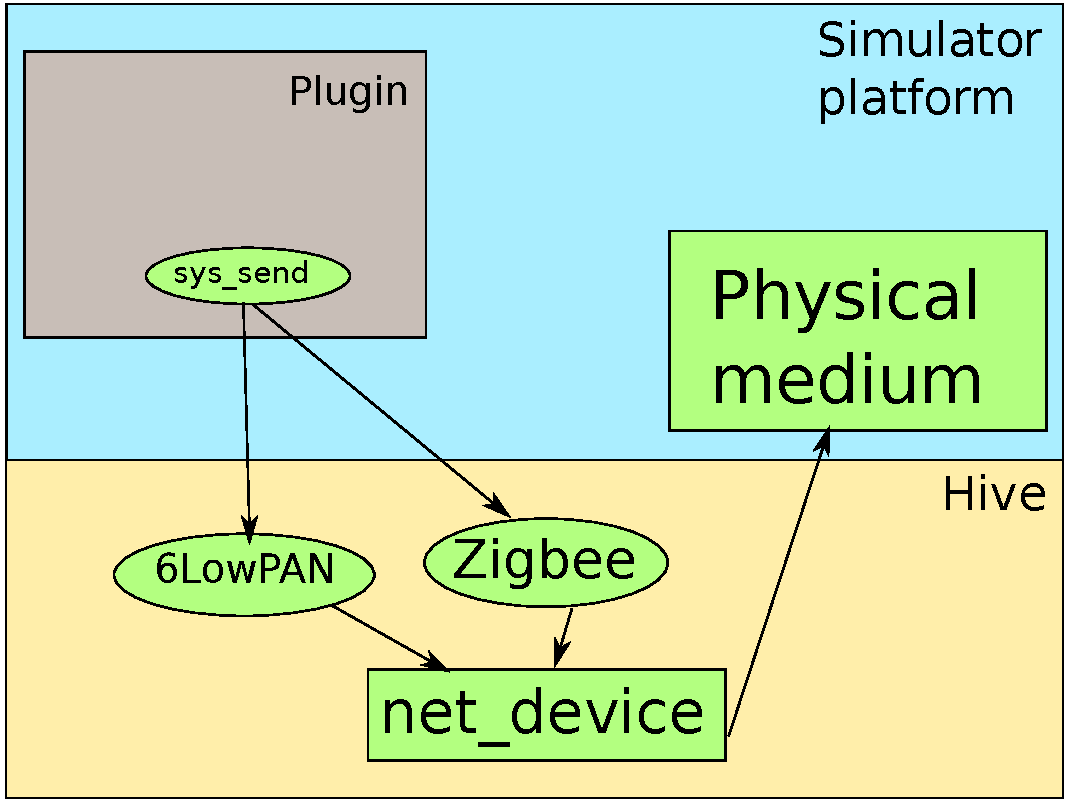
\includegraphics[scale=0.75]{img/networking.pdf}
    \caption{Network packet flow}
  \end{center}
\end{figure}

The flow of a network packet will start in the plugin. It will create a socket
using sys\_socket and will be able to send data using sys_sendto. In the
networking system a packet will be created in which the data from the buff
argument will be copied. This packet will be passed to the protocol for this
socket which will add the protocol specific headers to it based on internal
structures. When the protocol is done with the packet, it is passed to a
driver for a network device.

On a physical node, the network device driver will send the packet to the
destination node using WiFi, radio, etc... On the simulator platform, the
packet is passed back to the simulator which maintains a packet queus for each
node and will route the packet to the appropriate node.

On the receive side, the simulator periodically checks the receive packet
queues for nodes and sends a notification to the node to start processing it.
The packet will go through the network device driver, which will pass it to
the protocol which will pass it to the plugin after removing all headers.

\subsection{Scheduler}

Most of work on a wireless sensor node is triggered by an event. For example
we read the temperature sensor every 5 minutes, which is a timer event, or an
actual event happens on the node, for example a packet arrives.

The job of the scheduler is to provide a way to register for and notify of
events. It's split into two parts, a platform agnostic one and a platform
specific one. The platform agnostic part contains the API for users to use the
scheduler. It allows specifing callback for events or timers:

\begin{lstlisting}
typedef void (*callback_t)(void *arg);
void schedule_timer(struct scheduler *scheduler,
                    /* Timeout in miliseconds *?
                    int timeout, 
                    /* Callback function */
                    callback_t *cb, 
                    /* Argument to be passed to the callback */
                    void *arg);
\end{lstlisting}
The platform specific part contains the platform dependent implementation of
the scheduler. Each platform has a different implementation for timers so each
platform will have to implement its own version of this. For example linux has
timerfds, but an Atmega microcontroller has hardware timers. The scheduler
implementation for that platform will use what the platform provides.

The implementation of the scheduler on the simulation platform will be done
using libevent. The libevent API provides a mechanism to execute a callback
function when a specific event occurs on a file descriptor or after a timeout
has been reached. Furthermore, libevent also support callbacks due to signals
or regular timeouts. Libevent uses the event loop mechanisms provided by the
system on which it runs. This can be /dev/poll, kqueue, select, event ports,
poll, epoll.

\subsection{Accounting}

Everything that runs on a node consumes some power and the simulator will have
to reflect that in the battery level of the node. For example reading a sensor
will consume a small part of the battery while sending messages to a node will
consume much more power, depending on the distance of the target node from the
source node.

Every event on a simulated node will pass one or more times through the
scheduler. This will happen either a normal timer event or by the simulator
part of the driver for the component. If a timer expires, we call the callback
function which means the node is running some code and we will be able to
estimate how much battery it consumes based on the time the callback takes.
For a network packet we will be able to do the accouting when the packet
reaches the physical layer of the simulator where it will be able to compute
the power consumption to communicate with the target node.
